\documentclass[12pt]{article}

\usepackage{tikz}
\usepackage{mathtools}
\usepackage{caption}

\renewcommand{\theequation}{\arabic{section}.\arabic{equation}}

%opening
\title{A Recurrence Relation for Win Probabilities in Mafia}
\author{Caleb Vatral}

\begin{document}

\maketitle

\begin{abstract}
Mafia is an elimination based party game that deals with mob mentality. We divide into an uninformed majority against an informed minority. In this analysis we examine the most simple form of the game to develop a mathematical model for the probability of winning. We are able to find a recurrence relation for the probability and analyze some of its key features through numerical simulation.
\end{abstract}

\section{Basic Game}
\subsection{Game Rules}
In its simplest form, Mafia is an elimination based party game. Players are divided into two groups, the citizens and the mafia, by one referee. The group of all players is referred to as the town. The game divides into two phases: night and day. During the night phase, the town falls asleep. The mafia then awake and vote to kill one citizen. They then go back to sleep. The town awakes to find one player eliminated from the mafia strike. The town debates and votes to eliminate one player. The game then returns to night and loops in this way. The game ends when either all the mafia is eliminated, or all the citizens are eliminated.

\subsection{Strategic Game}
\subsubsection{Players and Groups}
\begin{itemize}
	\item There is a set, $\left<T\right>$, consisting of $T$ players. We refer to this set as the town.
	\item There exists  $\left<M\right>\subset\left<T\right>$ containing $M$ players who are considered mafia. We also make the restriction that $M < \frac{1}{2}T$, so that the mafia is a minority of players. 
	\item There exists  $\left<C\right>\subset\left<R\right>$ containing $T-M$ players who are considered citizens.
	\item There exists a person who shall be called the referee. The referee assigns players to specific subgroups, but is not a player themselves because the referee makes no decisions once the game has begun.
	\item We can effectively treat the game in a two player structure, with player one being $\left<M\right>$ and player two being $\left<C\right>$. 
\end{itemize}
\subsubsection{Information}
At the beginning of the game, each player is given the following information:
\begin{itemize}
	\item Each player is informed what subgroup they belong to, i.e. either a citizen or a mafia.
	\item Each member of the mafia is informed who all other mafia members are.
\end{itemize}

For $\left<M\right>$, the game is perfect information, as they are aware of the identity of all players. The rest of the game is constructed of decisions for these players. The remaining players represent $\left<C\right>$ and do not have perfect information, as the identity of any other players is not known. So in less mathematical terms, at the start of the game, $\left<M\right>$ is an informed minority and $\left<C\right>$ is an uninformed majority. However, by the end of the game, all players, either eliminated or remaining, have perfect information.

\subsubsection{Actions}

\begin{center}
	% Node styles
	\tikzset{
		% Two node styles for game trees: solid and hollow
		solid node/.style={circle,draw,inner sep=1.5,fill=black},
		hollow node/.style={circle,draw,inner sep=1.5}
	}
	\begin{tikzpicture}
	
	% Specify spacing for each level of the tree
	\tikzstyle{level 1}=[level distance=15mm,sibling distance=35mm]
	\tikzstyle{level 2}=[level distance=15mm,sibling distance=35mm]
	
	\node(0)[solid node,label=above:{$N\left(C,M\right)$}]{}
	child{node(0-1)[hollow node, label=left:{$D\left(C,M\right)$}]{}
		child{node(0-1-1)[solid node,label=below:{$N\left(C-1,M-1\right)$}]{} }
		child{node(0-1-2)[solid node,label=below:{$N\left(C-2,M\right)$}]{} }
	};
	% information sets
	\draw[dashed](0)to[out=0,in=-15](0-1-2);
	\draw[dashed](0)to[out=180,in=190](0-1-1);
	
	\end{tikzpicture}
	\captionof{figure}{A game tree of a recursive representation of the extensive form.}
\end{center}

\paragraph{Night Phase}
During the night phase of the game, $\left<M\right>$ makes one action. The group of mafia vote to eliminate one member of $\left<C\right>$. So the number of possible actions during the night phase is equal to the current size of $\left<C\right>$. We denote this action phase by $N\left(C,M\right)$.

The primary consequence associated with each of these actions is, of course, the elimination of the player. However, the other consequence is a change of probability and revelation of information. Elimination of a citizen raises the probability that a member of the mafia will be eliminated during the next day phase. Additionally, since the mafia eliminated the player, it is revealed to all players that the eliminated player was a citizen.

There is effectively no preference relation for the night phase, since the all members of $\left<C\right>$ are of equal utility to eliminate for the mafia.

\paragraph{Day Phase}
During the day phase of the game, there is a simultaneous action of both $\left<M\right>$ and $\left<C\right>$. Combined, this means the town, $\left<T\right>$, makes one action. The town votes democratically to eliminate one of its members. In the case of a tie vote, a random player is eliminated. So the number of possible moves during the day phase is equal to the current size of $\left<T\right>$. The interesting part about this action, however, is that only players with perfect information know how it changes the game. Members of the mafia know the role of the eliminated player, but citizens do not. We denote this action phase by $D\left(C,M\right)$.

The primary consequence associated with each of these actions is, again, the elimination of the player. Once again, a secondary consequence is the change in the probability of elimination of either mafia or citizens; however, as mentioned before, only players with perfect information are aware of this change.

The day phase also has an associated preference relation for each player subset. The relation denotes how each group prefers players to be eliminated. The preference relation for the mafia, $\prec_{\left<M\right>}$, sets the elimination of citizens strictly higher than the elimination of mafia. More formally: 
\begin{equation}
\forall i \in \left<C\right>, j \in \left<M\right> \rightarrow A_j \prec_{\left<M\right>} A_i
\end{equation}

The preference relation for the citizens, $\prec_{\left<C\right>}$, sets the elimination of mafia strictly higher than the elimination of citizens. More formally: 
\begin{equation}
\forall i \in \left<C\right>, j \in \left<M\right> \rightarrow A_i \prec_{\left<C\right>} A_j
\end{equation}

If the mafia outnumbers the citizens, then the day phase action will always follow $\prec_{\left<M\right>}$. However, since $\left<C\right>$ does not have perfect information, there is no way for them to determine how to pick their actions. So, the action made during the day phase may not follow $\prec_{\left<C\right>}$, even if the citizens outnumber the mafia.

\paragraph{Looping}
There are two major loops that occur in the extensive form. Both loops occur after the day phase action is taken to loop the game back to the night phase. This gives the game a recursive nature. The conditions of the recursion depend on the actions of the players, especially the actions of the town during the day phase. If a citizen is eliminated during the day phase, then a total of two citizens were eliminated during a single loop iteration. So the recursion is $N\left(C,M\right) \rightarrow N\left(C-2,M\right)$. If a mafia member was eliminated during the day phase, then one mafia and one citizen were eliminated during the loop cycle, and the recursion is $N\left(C,M\right) \rightarrow N\left(C-1,M-1\right)$.

The game ends when either all mafia or all citizens are eliminated. In terms of the recurrence, the game ends when we reach $N\left(0,M-k\right)$ or $N\left(C-k,0\right)$ where $k$ is some arbitrary number of passes rounds. However, the mafia has a slight advantage if the town picks their action democratically (as we assume). If the action is picked this way, then the mafia wins as soon as they attain a majority, i.e. $C-k<M-l$, where $k$ and $l$ are some arbitrary amount of eliminated players.

\subsection{Strategies}

For this analysis, we neglect any sort of psychological strategies. However, in its basic form, the game does not consist of much mathematical strategy. The mafia's preference relation equates the elimination of all citizens, so they will simply choose at random during the night phase. For the day phase, not all members of the town have perfect information, so picking who should be eliminated is random as well. In fact, if the day phase decision is not random, then it is more susceptible to the influence of those who have perfect information (i.e. the mafia). So when the town picks randomly, any player who opposes the decision must surely be mafia and should be eliminated.

Assume for a moment that there is a better strategy for the citizens than random. Since the mafia have perfect information, they can then force a random elimination by posing as citizens.

Assume for a moment that there is a better strategy for the mafia than random. Since the citizens are in the majority of the town, they can force a random elimination by some method of random assignment (die roll, etc.). The only consideration is when the mafia is in the majority, which already forces a win as discussed earlier.

Since random elimination is the best action profile for both groups, we can call it the Nash equilibrium.

Assuming random elimination is followed, we can model the probability of each recursive node in the extensive form:
\begin{equation}
P\left[N\left(C,M\right) \rightarrow N\left(C-2,M\right)\right]=\frac{T-M}{T}
\end{equation}
\begin{equation}
P\left[N\left(C,M\right) \rightarrow N\left(C-1,M-1\right)\right]=\frac{M}{T}
\end{equation}

Let $w\left(T,M\right)$ be the probability of $\left<M\right>$ winning the game. From the transition probabilities (eq 3.3, 3.4) derived from random elimination strategies, we can write a recursive relation for $w\left(T,M\right)$:
\begin{equation}
	w\left(T,M\right) =
	\begin{cases*}
		0 & if $M=0$ \\
		1 & if $M>T-M$ \\
		\frac{T-M}{T}w\left(T-2,M\right) + \frac{M}{T}w\left(T-2,M-1\right) & Else
	\end{cases*}
\end{equation}

\subsection{Conclusions}
\begin{center}
	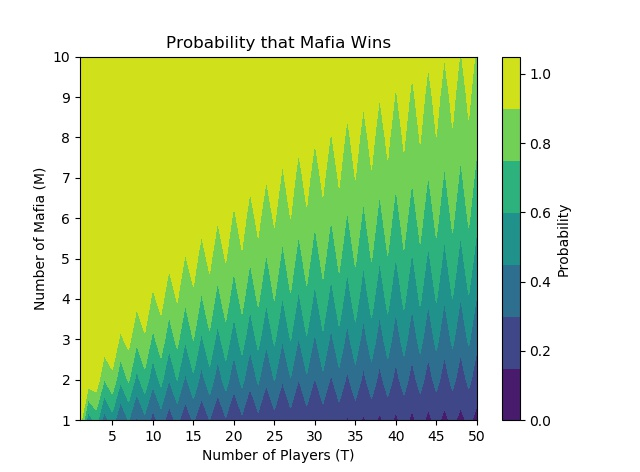
\includegraphics[width = \linewidth]{images/simple/simulation_results}
	\captionof{figure}{A numerical simulation of the probability that the mafia wins the game, $w\left(T,M\right)$.}
\end{center}

A simulation was run to test the recursive probability formula (eq 3.5). The simulation compared initial values of $T$ between 1 and 50, and initial values of $M$ between 1 and 10. A few conclusions can be drawn easily from the results.

First, the win probabilities are heavily dependent on the initial conditions, which is to be expected. However, the probabilities do no change linearly with these parameters. As $T$ increases, the amount that $M$ has to increase to maintain equal probability decreases. So, there must be some non-linear relationship between $M$ and $T$ in order to make the probability of the mafia winning equal to the probability of the citizens winning.

Next, the probabilities are heavily reliant on the parity of $T$. This is suggested by the jagged oscillation of the contour lines. To test this fully, the numeric simulation was run again, this time for fixed 1 mafia member.

\begin{center}
	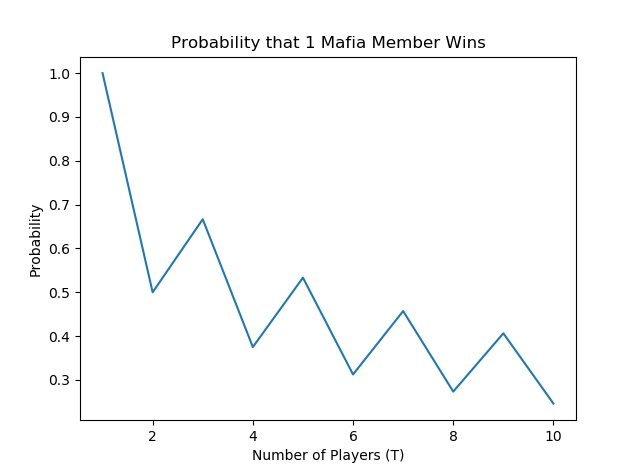
\includegraphics[width = \linewidth]{images/simple/simulation_results_1}
	\captionof{figure}{A numerical simulation of the probability that 1 mafia member wins the game, $w\left(T,1\right)$.}
\end{center}

From this plot, it is easy to see the dependency of probability on parity. An odd amount of total players gives the mafia member higher probabilities. This is a bit counterintuitive since one would expect that raising the amount of players always lowers the mafia member's probabilities. However, if $T$ is raised by 1 to an odd value, the probability actually increases. 

More work should be done to try to solve the recurrence relation and determine a closed form solution to the probability of winning. Additionally, more work has to be done to analyze other complexities of the game such as psychological aspects and additional roles not discussed here.

\rule{\linewidth}{1pt}

\end{document}
